\chapter{Probleemanalyse}
\label{hoofdstuk:probleemanalyse}
\textbf{In dit hoofdstuk komt de afbakening en het onderzoeksonderwerp aan de orde. Juist omdat de opdracht zich plaats vindt in een dergelijke complexe omgeving met een ingewikkelde centrale vraag is het belangrijk om hier bij stil te staan. Dit hoofdstuk is voornamelijk bedoeld om het onderzoek te definiëren, maar ook om grenzen te stellen aan de rijkwijdte van het onderzoek.}

\medskip 

\section{De aanleiding}
Deze opdracht is ontstaan vanuit de finance afdeling in het afgelopen jaar. Deze handelt registrerend en controlerend ten behoeve van de \gls{geldgoederen}. De intern beschikkende afdelingen –- inkoop en verkoop --– werken nauw samen met finance voor de bewaking en afdekking van vreemde valuta. Het afdekken van vreemde valuta is een maatregel van hedging. Hedging kan onder andere gebruikt worden om \gls{valuta}, \gls{rente}, en \gls{koers} te verminderen (zie de begrippenlijst voor definitie). Deze drie soorten risico's komen hierna terug als de afkorting: \gls{fx}. Het management en de afdeling finance hebben samen een voorkeur voor een formeel vastgelegd beleid voor het geldmiddelenbeheer en zochten hiervoor een passende afstudeerder. Het vastleggen van het geldmiddelenbeheer is verbonden aan de Administratieve Organisatie en de Interne Beheersingsmaatregelen. Deze connectie zit in de maatregelen die de organisatie
%\makebox[\textwidth][s]{}

\vfill
\begin{center}
  \makebox[\textwidth]{
\includegraphics[width=1.09\paperwidth]{scn046}}
\end{center}

\noindent
van SFC treft om de \gls{geldgoederen} te beheersen. Klip en klaar is het centrale probleem gegrond in de waardering van financiële middelen. De inkopen en verkopen zijn vaak niet in dezelfde valuta, dit heeft als gevolg dat de brutomarge enorm kan schommelen. Hedging speelt hierbij de rol dat deze schommelingen bedaard worden door een aantal organisatorische maatregelen. Om deze maatregelen in kaart te brengen herschrijft de afstudeerder de AOIB van de primaire processen met het doel van de opdrachtgever in het achterhoofd. Het doel is zwart-op-wit te hebben welke afspraken en maatregelen de organisatie treft om de beheersing te vergroten. Deze maatregelen moeten zo nauw mogelijk aansluiten op de werkelijkheid, de afstudeerder gaat deze aansluiting onderzoeken en uitwerken door het gesprek aan te gaan en de gestelde normen te toetsen aan de werkelijkheid. 

\section{Probleemomschrijving}
\label{beschr:problemen}
De AOIB bij Seafood Connection is verouderd, dit komt doordat er nieuwe afdelingen zijn ontstaan, er nieuwe functies zijn gecreëerd of zijn veranderd, en dat het organogram veranderd is. Het bedrijf is sinds de laatste update van de AOIB verdubbeld qua omzet en personeel. Een update is dus hoognodig om te voorkomen dat de vastgelegde AOIB niet overeenkomt met de werkelijkheid. Het vastleggen van de AOIB is niet meer dan een momentopname van de organisatie, het hebben van een goed omschreven AO leidt dus niet automatisch tot \gls{intbeh}. Het denken over, en vastleggen van deze AOIB kan wel enige bewustwording stimuleren zodat er kritisch gaat nagedacht worden over hoe de organisatie wordt ingericht. \citep{bivpraktijk}

Juist door deze verouderde AO is er een verschil tussen de daadwerkelijke bedrijfsprocessen en de formele vastlegging hiervan. 
Het knelpunt hier is de vastlegging van de organisatorische maatregelen rond de financiële geldstromen. Zoals eerder beschreven in paragraaf \ref{beschr:activiteiten} haalt Seafood Connection haar bestaansgrond uit het feit dat er op grote schaal wordt ingekocht en verkocht op een internationale markt. De \gls{geldgoederen} is een cruciaal deel van de bedrijfsvoering die in de bestaande versie van de AOIB niet uitgebreid en doordacht is vastgelegd. \citep{aoibsfc}

De organisatorische maatregelen rond de financiële geldstromen komen voort uit de AOIB, de aflegging van het beleid over financiële geldstromen is dus onlosmakelijk van de administratieve organisatie. 

Momenteel is er nog niet een vastgelegd document omtrent de \textit{\gls{treasury}} dat aansluit op het beleid rondom geldzaken. Treasurybeleid is de manier waarop een onderneming haar \textit{treasures} (of ook: schatten) beheert. De praktische invulling van het treaurybeleid wordt omschreven in het door de management opgestelde \gls{treasuryletter}. 
Deze letter is \textbf{intern} gericht door in kaart te brengen hoe de verschillende processen rond de financiële beheersing horen te functioneren, er wordt bijvoorbeeld beschreven wie welke functie heeft in het \gls{geldgoederen} en welke controles daarop uitgevoerd worden. \\
Ook is de \gls{treasuryletter} \textbf{extern} gericht aan stakeholders door de verantwoording die wordt afgelegd, door het management, over het geldbeheer. \citep{jans}

\newpage
In deze rapportage wordt de volgende definitie gehanteerd voor de term \gls{treasuryletter}: 

\begin{displayquote}
De \gls{treasuryletter} is een door het management opgesteld rapport waarin de bevoegdheden, verantwoordelijkheden, toezichtmaatregelen, de sturing, en beheersing geformuleerd worden ten aanzien van financiële vermogenswaarden, financiële geldstromen, financiële posities en de hieraan verbonden risico’s. \\
\citep{jans,buunk} \label{def:treasury}
\end{displayquote}
\noindent
Zie ook \hyperlink{bij:treasury}{bijlage 1} voor een overzichtelijke uitwerking van het begrip \gls{treasuryletter}.

De treasuryfunctie is een essentieel deel van alle primaire processen bij Seafood Connection door de grote aanwezigheid van vreemde valuta in zowel het inkoop- als verkoopproces. Figuur \ref{fig:primairproces} laat zien hoe de primaire processen verband houden met elkaar. Enkele communicatiestromen zijn hier ook weergegeven, namelijk de inkopers die voor het betalen van een levering in een andere valuta aan de finance-afdeling het verzoek sturen om euro's te verkopen voor bijvoorbeeld dollars. De verkopers vragen aan de finance-afdeling of zij vreemde valuta willen inkopen om de brutomarge vast te zetten.

Samenvattend worden de huidige bestaande organisatorische maatregelen en processen in kaart gebracht. Daarnaast is het management van SFC bewust dat er op een navolgbare en verantwoordelijke manier omgegaan moet worden met financiële middelen; immers handelt het bedrijf met een uitputbare hoeveelheid vreemde valuta en is er een hoge mate van liquiditeit vereist om het bestaan van het bedrijf in de toekomst te kunnen garanderen. De \gls{treasuryletter} is onlosmakelijk verbonden met de AOIB, het is daarom noodzakelijk dit product pas wordt opgesteld wanneer de AO weer aansluit op de werkelijkheid \citep{watisonderzoek,buunk,financiering}.

\begin{figure}[!ht]
    \centering
    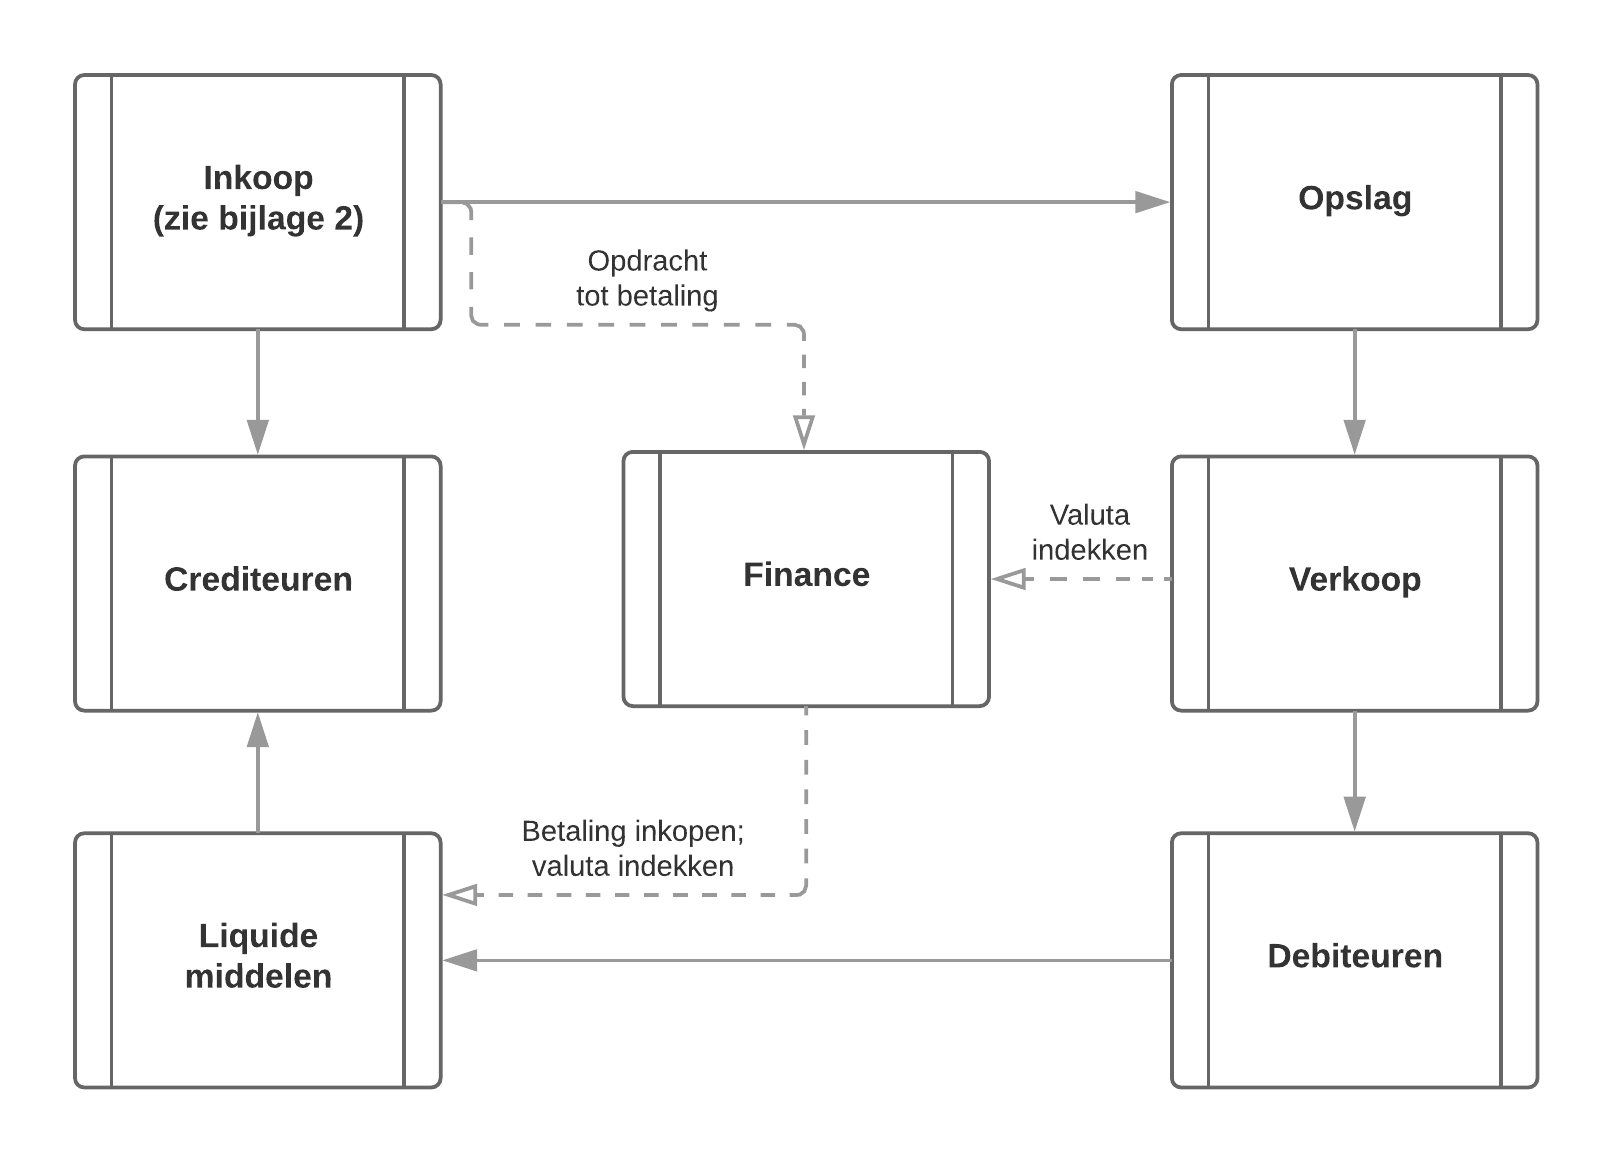
\includegraphics[width=0.8\textwidth]{primairproces}
    \caption{Globaal overzicht van de primaire processen \citep{bivpraktijk}}
    \label{fig:primairproces}
\end{figure}

\subsection{De doelstelling}
Het doel van de afstudeerstage is dat de afstudeerder de bestaande AOIB herschrijft waarbij vervolgens een zogenaamde \gls{treasuryletter} opstelt (zie paragraaf \ref{def:treasury}). Deze twee producten zijn \textit{deliverables}, met andere woorden: deze producten komen niet direct voort uit de centrale vraagstelling. de update van de AOIB en de  \gls{treasuryletter} vloeien voort vanuit de uitwerking van het interne betrouwbaarheidssysteem. Beide deliverables zijn te vinden in bijlages 4 en 5. 
Het interne betrouwbaarheidssysteem wordt onder de loep genomen waarbij vooral gekeken wordt naar de sterke en zwakke aspecten van de organisatorische inrichting. In de \gls{treasuryletter} legt het management verantwoording af over het kas- en geldmiddelenbeheer en dus ook over hoe \gls{fx}-risico wordt bestreden. Deze aflegging van de verantwoording over de financiële middelen moet in lijn zijn met de getroffen, organisatorische maatregelen en de manier waarop het management idealistisch de geldstromen bewaakt en monitort. Het management geeft zelf aan dat het opstellen van deze \gls{treasuryletter} een hoognodig deel is van het onderzoek, aangezien er al een bestaande AO aanwezig is en dat het kasmanagement, hoewel grotendeels geautomatiseerd, nog niet formeel is vastgelegd. Bij de uitwerking van de update van de AO wordt door de organisatorische veranderingen (beschreven in paragraaf \ref{beschr:problemen}) ook rekening gehouden met nieuwe afdelingen, veranderde afdelingen, nieuwe organisatiestructuren, afdelingen die gericht zijn op nieuwe producten en nieuwe markten.

Het doel is om de bestaande AOIB in brede zin in kaart te brengen. Nadenken over de structuren en maatregelen, zoals dat in een AO-beschrijving gebeurt, is voor veel bedrijven belangrijk om niet alleen te kunnen groeien in de toekomst, maar ook om het bestaan van de onderneming enigszins te kunnen garanderen en om te toetsen of er niet ongeoorloofd middelen uit de onderneming wegvloeien.


\subsection{De hoofdvraag}
Op basis van het voorgaande luidt de centrale hoofdvraag als volgt:

\smallskip
\noindent
\begin{center}
{\large{Wat is de kwaliteit van het interne betrouwbaarheidssysteem bij de primaire processen van Seafood Connection en hoe kan dit bijdragen dat er op een navolgbare en verantwoordelijke manier wordt omgegaan met vreemde valuta?}} 
%33 woorden. Alle belangrijke kenmerken: AOIB (soort: interne betrouwbaarheid, alleen primaire processen, Seafood Connection, doel van treasury, rol van AO in omgang van vreemde valuta)
\end{center}

Het bredere doel van het onderzoek is om een formele vastlegging van de administratieve organisatie en het treasurybeleid op tafel te krijgen. Hiermee wil de opdrachtgever bereiken dat de vastgelegde AOIB aansluit op de daadwerkelijke situatie, of ook wel dat de organisatie formeel zwart-op-wit is vastgelegd. Het opstellen van de \gls{treasuryletter} is van grote waarde voor de opdrachtgever omdat de \gls{geldgoederen} een cruciaal deel van de bedrijfsvoering is die op het moment niet uitgebreid en doordacht is vastgelegd. Dit onderzoek besteed een bijzondere aandacht aan het primaire proces van Seafood Connection B.V. Hier worden onder verstaan: de inkoop-, voorraad-, en verkoopafdeling(en). 

\newpage
\subsection{De deelvragen}
Om de hoofdvraag te beantwoorden wordt gebruik gemaakt van het zogenaamde model van COSO Internal Control Framework. Veel onderzoeken die met interne betrouwbaarheid te maken hebben passen dit model toe. De hierbij horende deelvragen die ieder zullen helpen bij het beantwoorden van de hoofdvraag, zijn:

\begin{enumerate}
    \item Wat zijn de sterke en zwakke punten van de controle-omgeving bij Seafood Connection?
    \item Welke betrouwbaarheidsrisico's zijn te onderkennen bij Seafood Connection bij de primaire processen van de onderneming?
    \item Welke preventieve en repressieve maatregelen worden getroffen om de \gls{ic} in stand te houden?
    \item Welke maatregelen zijn getroffen om er voor te zorgen dat er voldoende informatie en communicatie is binnen de organisatie?
    \item Hoe wordt er voor gezorgd dat het interne betrouwbaarheidssysteem regelmatig geëvalueerd en gemonitord wordt?
\end{enumerate}

\section{Theoretische ondersteuning onderzoek}
\label{hoofdstuk:theoretischeondersteuning}
De uitwerking van de deelvragen wordt gedaan aan de hand van het COSO Internal Control Framework \citep{COSOsummery}. De daadwerkelijke invulling hiervan wordt aan de hand van de uiteenzetting in de literatuur van \citet{bivpraktijk} en die van \citet{bivperspectief} verder verdiepend uitgewerkt. 

Voor de uitwerking van het COSO-model wordt ook gesteund op de theorie van Starreveld waarin per \gls{typologie} onder andere wordt uitgewerkt welke preventieve en repressieve maatregelen verwacht worden \citep{jans,financiering,buunk}. Door middel van deze theorie is het mogelijk een theoretisch kader op te stellen door verschillende typologieën te combineren. 

\begin{figure}[!h]
    \centering
    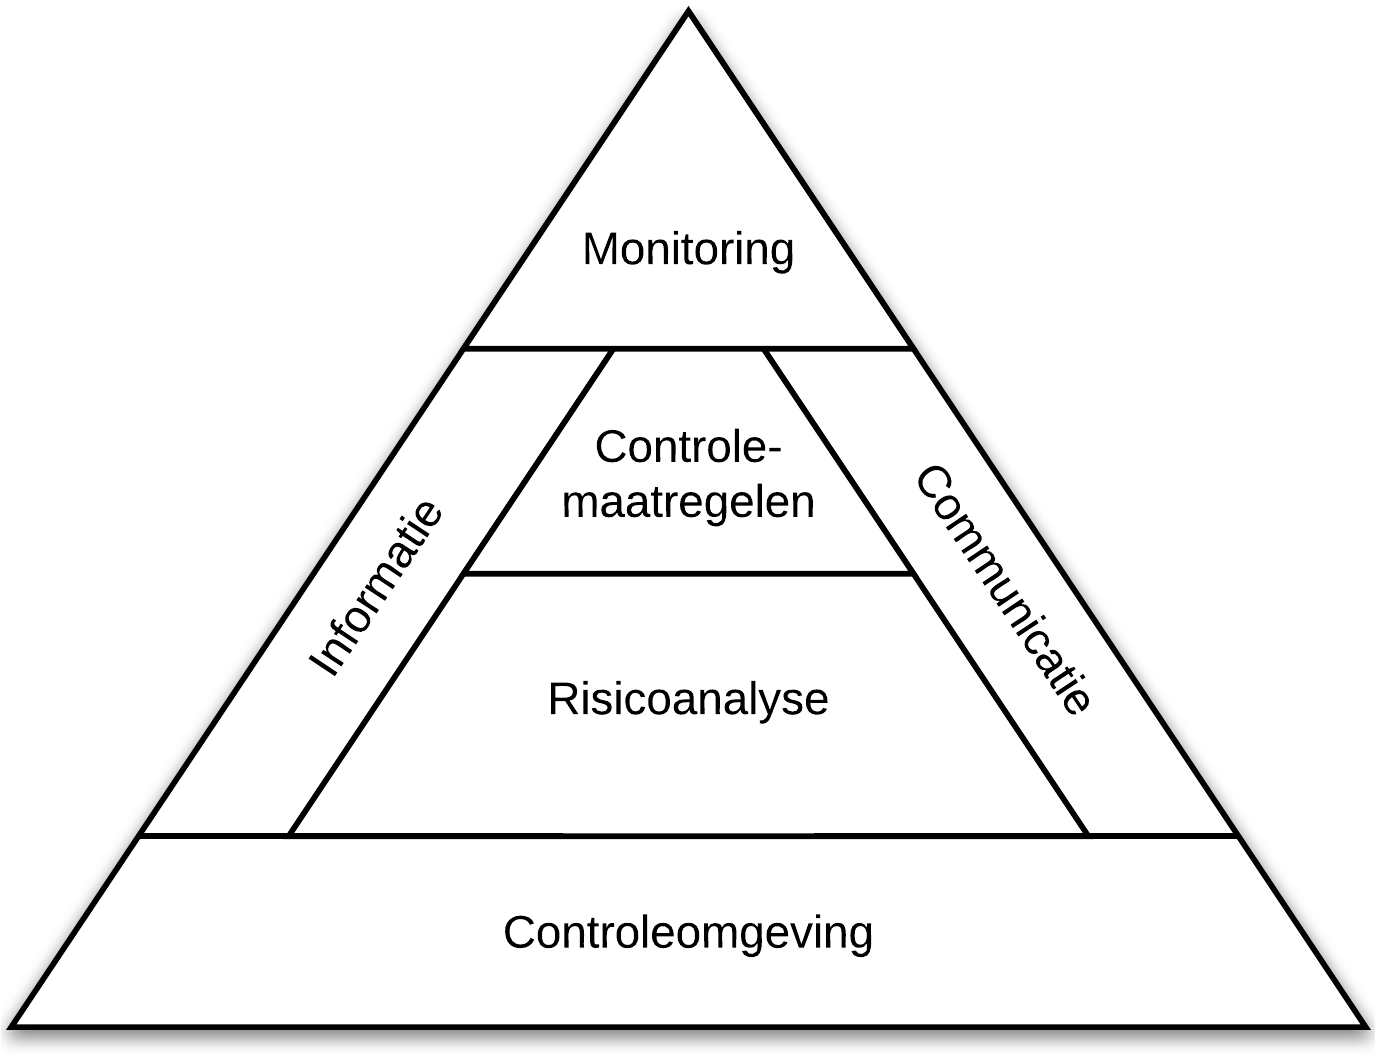
\includegraphics[width=0.6\textwidth]{coso}
    \caption{Het COSO Internal Control Framework \citep{COSOsummery}}
    \label{fig:coso}
\end{figure}

Samenvattend wordt het COSO-model uitgewerkt om de organisatie als geheel te kunnen omschrijven en om de centrale hoofdvraag te kunnen beantwoorden. De uitwerkingen van de \gls{biv} van \citet{bivperspectief} en van \citet{bivpraktijk} worden gebruikt voor de interpretatie van het COSO-model. Voor de specifieken van elke laag in het COSO-model en als onderbouwing en uitwerking van de verschillende afdelingen en processen worden de boeken gebruikt omtrent procesbeheersing en de specifieke relevante onderwerpen. \citep{internebeheersing,jans,financiering,buunk}

Deze onderzoeksopdracht valt onder de noemer `betrouwbaarheid breed'. Deze is gericht op het inrichten van het \gls{intbet}ssysteem in het algemeen. Deze opdracht wordt voornamelijk toegepast bij organisaties die sterk aan het groeien zijn en die graag willen weten of de bestaande \gls{ic}maatregelen nog voldoende zijn. Een veel voorkomende opdracht hierbij is dat het bestaande AOIB handboek verouderd is. \citep{bivpraktijk}